\documentclass[11pt,a4paper]{report}
\usepackage[textwidth=37em,vmargin=30mm]{geometry}
\usepackage{calc,xunicode,amsmath,amssymb,paralist,enumitem,tabu,booktabs,datetime2,xeCJK,xeCJKfntef,listings}
\usepackage{tocloft,fancyhdr,tcolorbox,xcolor,graphicx,eso-pic,xltxtra,xelatexemoji}

\newcommand{\envyear}[0]{2025}
\newcommand{\envdatestr}[0]{2025-07-06}
\newcommand{\envfinaldir}[0]{webdb/2025/20250706/final}

\usepackage[hidelinks]{hyperref}
\hypersetup{
    colorlinks=false,
    pdfpagemode=FullScreen,
    pdftitle={Web Digest - \envdatestr}
}

\setlength{\cftbeforechapskip}{10pt}
\renewcommand{\cftchapfont}{\rmfamily\bfseries\large\raggedright}
\setlength{\cftbeforesecskip}{2pt}
\renewcommand{\cftsecfont}{\sffamily\small\raggedright}

\setdefaultleftmargin{2em}{2em}{1em}{1em}{1em}{1em}

\usepackage{xeCJK,xeCJKfntef}
\xeCJKsetup{PunctStyle=plain,RubberPunctSkip=false,CJKglue=\strut\hskip 0pt plus 0.1em minus 0.05em,CJKecglue=\strut\hskip 0.22em plus 0.2em}
\XeTeXlinebreaklocale "zh"
\XeTeXlinebreakskip = 0pt


\setmainfont{Brygada 1918}
\setromanfont{Brygada 1918}
\setsansfont{IBM Plex Sans}
\setmonofont{JetBrains Mono NL}
\setCJKmainfont{Noto Serif CJK SC}
\setCJKromanfont{Noto Serif CJK SC}
\setCJKsansfont{Noto Sans CJK SC}
\setCJKmonofont{Noto Sans CJK SC}

\setlength{\parindent}{0pt}
\setlength{\parskip}{8pt}
\linespread{1.15}

\lstset{
	basicstyle=\ttfamily\footnotesize,
	numbersep=5pt,
	backgroundcolor=\color{black!5},
	showspaces=false,
	showstringspaces=false,
	showtabs=false,
	tabsize=2,
	captionpos=b,
	breaklines=true,
	breakatwhitespace=true,
	breakautoindent=true,
	linewidth=\textwidth
}






\newcommand{\coverpic}[2]{
    % argv: itemurl, authorname
    Cover photo by #2~~(\href{#1}{#1})
}
\newcommand{\makeheader}[0]{
    \begin{titlepage}
        % \newgeometry{hmargin=15mm,tmargin=21mm,bmargin=12mm}
        \begin{center}
            
            \rmfamily\scshape
            \fontspec{BaskervilleF}
            \fontspec{Old Standard}
            \fontsize{59pt}{70pt}\selectfont
            WEB\hfill DIGEST
            
            \vfill
            % \vskip 30pt
            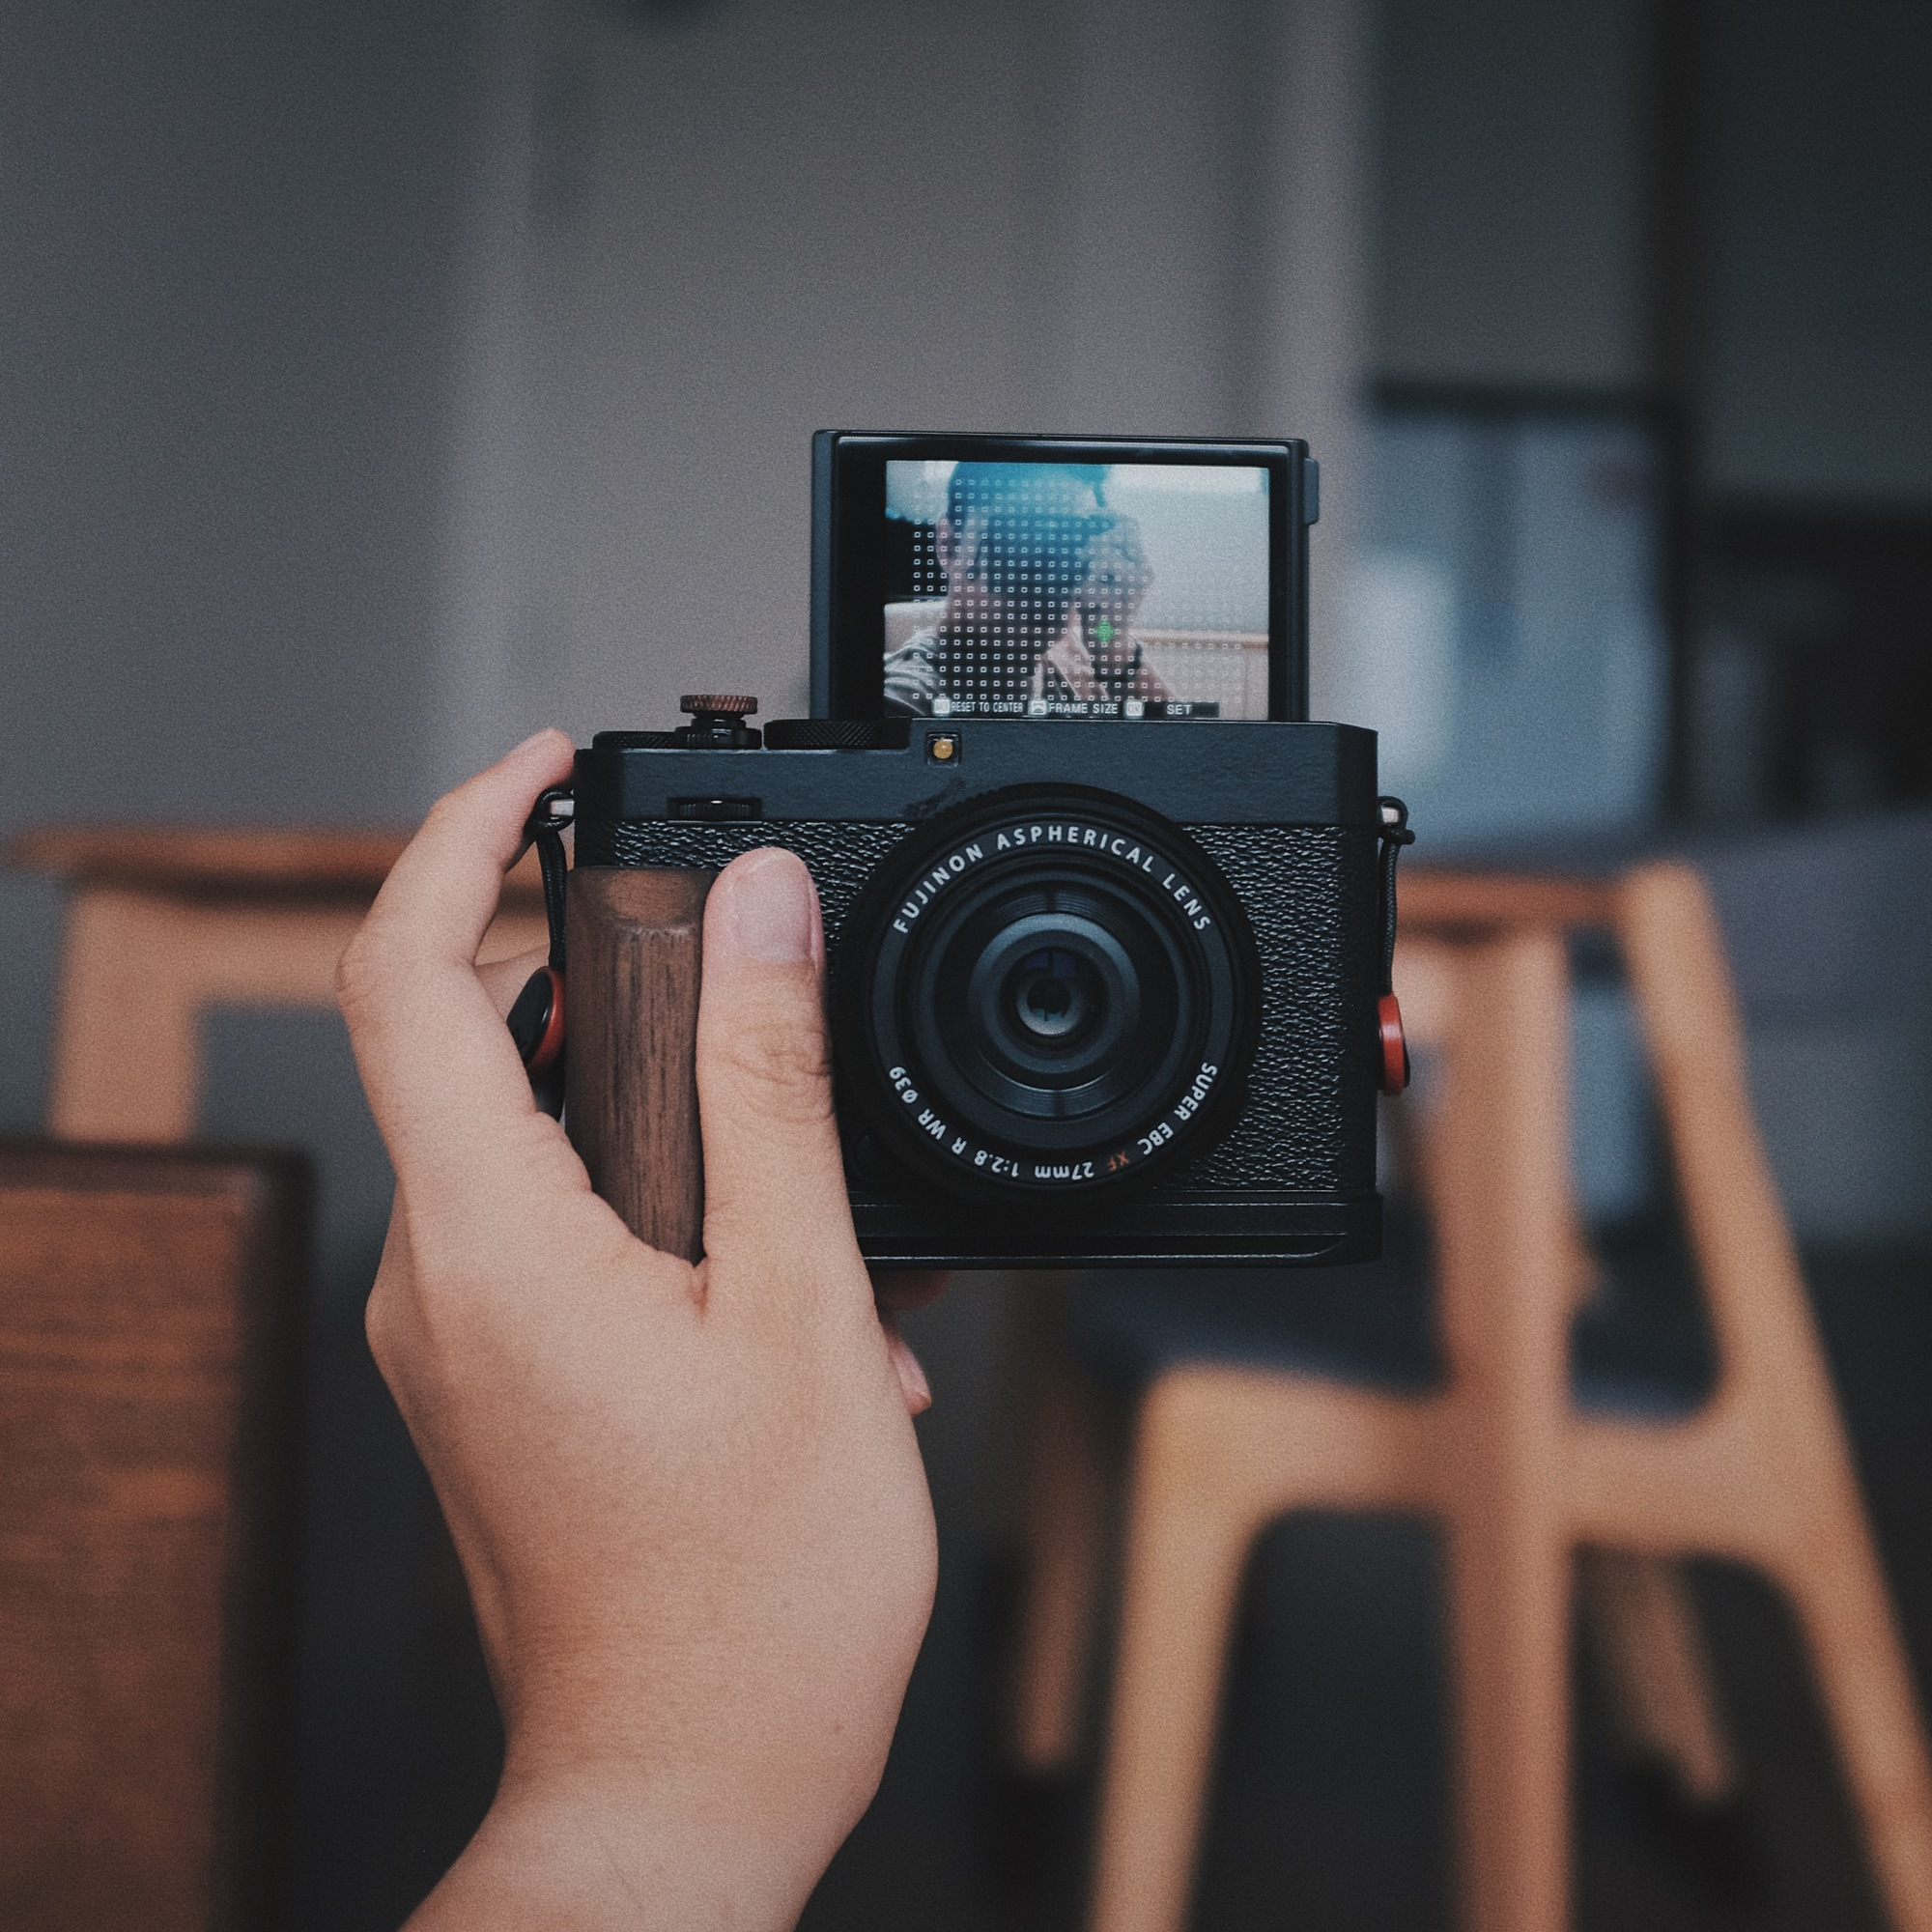
\includegraphics[width=\linewidth]{\envfinaldir/coverpic-prod.jpg}\par
            % \vskip 30pt
            \vfill

            \normalsize\rmfamily\scshape
            \copyright{} The Web Digest Project \hfill\large \envdatestr
        \end{center}
    \end{titlepage}
    % \restoregeometry
}
\newcommand{\simplehref}[1]{%
    \textcolor{blue!80!green}{\href{#1}{#1}}%
}
\renewcommand{\contentsname}{\center\Huge\sffamily\bfseries Contents\par\vskip 20pt}
\newcounter{ipartcounter}
\setcounter{ipartcounter}{0}
\newcommand{\ipart}[1]{
    % \vskip 20pt
    \clearpage
    \stepcounter{ipartcounter}
    \phantomsection
    \addcontentsline{toc}{chapter}{#1}
    % \begin{center}
    %     \Huge
    %     \sffamily\bfseries
    %     #1
    % \end{center}
    % \vskip 20pt plus 7pt
}
\newcounter{ichaptercounter}
\setcounter{ichaptercounter}{0}
\newcommand{\ichapter}[1]{
    % \vskip 20pt
    \clearpage
    \stepcounter{ichaptercounter}
    \phantomsection
    \addcontentsline{toc}{section}{\numberline{\arabic{ichaptercounter}}#1}
    \begin{center}
        \Huge
        \sffamily\bfseries
        #1
    \end{center}
    \vskip 20pt plus 7pt
}
\newcommand{\entrytitlefont}[1]{\subsection*{\raggedright\Large\sffamily\bfseries#1}}
\newcommand{\entryitemGeneric}[2]{
    % argv: title, url
    \parbox{\linewidth}{
        \entrytitlefont{#1}\par\vskip 5pt
        \footnotesize\ttfamily\mdseries
        \simplehref{#2}
    }\vskip 11pt plus 11pt minus 1pt
}
\newcommand{\entryitemGithub}[3]{
    % argv: title, url, desc
    \parbox{\linewidth}{
        \entrytitlefont{#1}\par\vskip 5pt
        \footnotesize\ttfamily\mdseries
        \simplehref{#2}\par\vskip 5pt
        \small\rmfamily\mdseries#3
    }\vskip 11pt plus 11pt minus 1pt
}
\newcommand{\entryitemAp}[3]{
    % argv: title, url, desc
    \parbox{\linewidth}{
        \entrytitlefont{#1}\par\vskip 5pt
        \footnotesize\ttfamily\mdseries
        \simplehref{#2}\par\vskip 5pt
        \small\rmfamily\mdseries#3
    }\vskip 11pt plus 11pt minus 1pt
}
\newcommand{\entryitemHackernews}[3]{
    % argv: title, hnurl, rawurl
    % \parbox{\linewidth}{
    %     \entrytitlefont{#1}\par\vskip 5pt
    %     \footnotesize\ttfamily\mdseries
    %     \simplehref{#3}\par
    %     \textcolor{black!50}{\href{#2}{#2}}
    % }\vskip 11pt plus 11pt minus 1pt
    \begin{minipage}{\linewidth}
            \entrytitlefont{#1}\par\vskip 5pt
            \footnotesize\ttfamily\mdseries
            \simplehref{#3}\par
            \textcolor{black!50}{\href{#2}{#2}}
    \end{minipage}\par\vskip 11pt plus 11pt minus 1pt
}







\begin{document}

\makeheader

\tableofcontents\clearpage




\ipart{Developers}
\ichapter{Hacker News}
\entryitemTwoLinks{The Prime Reasons to Avoid Amazon}{https://news.ycombinator.com/item?id=44475297}{https://blog.thenewoil.org/the-prime-reasons-to-avoid-amazon}

\entryitemTwoLinks{Seine reopens to Paris swimmers after century-long ban}{https://news.ycombinator.com/item?id=44474297}{https://www.lemonde.fr/en/france/article/2025/07/05/seine-reopens-to-paris-swimmers-after-century-long-ban\_6743058\_7.html}

\entryitemTwoLinks{Local-First Software Is Easier to Scale}{https://news.ycombinator.com/item?id=44473590}{https://elijahpotter.dev/articles/local-first\_software\_is\_easier\_to\_scale}

\entryitemTwoLinks{macOS Icon History}{https://news.ycombinator.com/item?id=44473400}{https://basicappleguy.com/basicappleblog/macos-icon-history}

\entryitemTwoLinks{'Positive review only': Researchers hide AI prompts in papers}{https://news.ycombinator.com/item?id=44473319}{https://asia.nikkei.com/Business/Technology/Artificial-intelligence/Positive-review-only-Researchers-hide-AI-prompts-in-papers}

\entryitemTwoLinks{Local-first software (2019)}{https://news.ycombinator.com/item?id=44473135}{https://www.inkandswitch.com/essay/local-first/}

\entryitemTwoLinks{Europe's first geostationary sounder satellite is launched}{https://news.ycombinator.com/item?id=44472992}{https://www.eumetsat.int/europes-first-geostationary-sounder-satellite-launched}

\entryitemTwoLinks{Problems the AI industry is not addressing adequately}{https://news.ycombinator.com/item?id=44471695}{https://www.thealgorithmicbridge.com/p/im-losing-all-trust-in-the-ai-industry}

\entryitemTwoLinks{A 37-year-old wanting to learn computer science}{https://news.ycombinator.com/item?id=44471190}{https://initcoder.com/posts/37-year-old-learning-cs/}

\entryitemTwoLinks{Stop Killing Games}{https://news.ycombinator.com/item?id=44470632}{https://www.jeffgeerling.com/blog/2025/you-will-own-nothing-and-be-happy-stop-killing-games-0}

\entryitemTwoLinks{Why Tesla's cars keep crashing}{https://news.ycombinator.com/item?id=44470503}{https://www.theguardian.com/technology/2025/jul/05/the-vehicle-suddenly-accelerated-with-our-baby-in-it-the-terrifying-truth-about-why-teslas-cars-keep-crashing}

\entryitemTwoLinks{Why AO3 Was Down}{https://news.ycombinator.com/item?id=44469650}{https://www.reddit.com/r/AO3/s/67nQid89MW}

\entryitemTwoLinks{OBBB signed: Reinstates immediate expensing for U.S.-based R\&D}{https://news.ycombinator.com/item?id=44469124}{https://www.kbkg.com/feature/house-passes-tax-bill-sending-to-president-for-signature}

\entryitemTwoLinks{Nvidia won, we all lost}{https://news.ycombinator.com/item?id=44468175}{https://blog.sebin-nyshkim.net/posts/nvidia-is-full-of-shit/}

\entryitemTwoLinks{Everything around LLMs is still magical and wishful thinking}{https://news.ycombinator.com/item?id=44467949}{https://dmitriid.com/everything-around-llms-is-still-magical-and-wishful-thinking}

\entryitemTwoLinks{Being too ambitious is a clever form of self-sabotage}{https://news.ycombinator.com/item?id=44467912}{https://maalvika.substack.com/p/being-too-ambitious-is-a-clever-form}

\entryitemTwoLinks{The story behind Caesar salad}{https://news.ycombinator.com/item?id=44467312}{https://www.nationalgeographic.com/travel/article/story-behind-caesar-salad}

\entryitemTwoLinks{Eight dormant Satoshi-era Bitcoin wallets reactivated after 14 yrs}{https://news.ycombinator.com/item?id=44466896}{https://twitter.com/WatcherGuru/status/1941167512491864554}

\entryitemTwoLinks{Sleeping beauty Bitcoin wallets wake up after 14 years to the tune of \$2B}{https://news.ycombinator.com/item?id=44466888}{https://www.marketwatch.com/story/sleeping-beauty-bitcoin-wallets-wake-up-after-14-years-to-the-tune-of-2-billion-79f1f11f}

\entryitemTwoLinks{Air pollution may contribute to development of lung cancer in never-smokers}{https://news.ycombinator.com/item?id=44466838}{https://today.ucsd.edu/story/air-pollution-may-contribute-to-development-of-lung-cancer-in-never-smokers-new-study-finds}


\ipart{Developers~~~~(zh-Hans)}
\ichapter{Solidot}
\entryitemGeneric{\hskip 0pt{}微软 XBox 业务高管建议被裁员的员工用 AI 管理情绪}{https://www.solidot.org/story?sid=81729}

\entryitemGeneric{\hskip 0pt{}美国面临其历史上最大规模的人才流失}{https://www.solidot.org/story?sid=81728}

\entryitemGeneric{\hskip 0pt{}善用表情符号能在交流中给对方留下好印象}{https://www.solidot.org/story?sid=81727}

\entryitemGeneric{\hskip 0pt{}《圣歌》服务器将于 2026 年 1 月关闭}{https://www.solidot.org/story?sid=81726}

\entryitemGeneric{\hskip 0pt{}云南甘棠箐遗址出土 30 万年前木质工具}{https://www.solidot.org/story?sid=81725}

\entryitemGeneric{\hskip 0pt{}科学家警告美国可能会失去一代人才}{https://www.solidot.org/story?sid=81724}

\entryitemGeneric{\hskip 0pt{}空气污染和传统草药与肺癌相关}{https://www.solidot.org/story?sid=81723}

\entryitemGeneric{\hskip 0pt{}挪威六月电动汽车占总销量的 96.9\% }{https://www.solidot.org/story?sid=81722}

\entryitemGeneric{\hskip 0pt{}Stop Killing Games 运动吸引了逾百万人签名}{https://www.solidot.org/story?sid=81721}

\entryitemGeneric{\hskip 0pt{}2024 年发表的医学论文摘要七分之一可能是 AI 完成的}{https://www.solidot.org/story?sid=81720}

\entryitemGeneric{\hskip 0pt{}Clothoff 试图支配深度伪造色情}{https://www.solidot.org/story?sid=81719}

\entryitemGeneric{\hskip 0pt{}基因组测序揭示古埃及人祖先}{https://www.solidot.org/story?sid=81718}

\entryitemGeneric{\hskip 0pt{}海绵结构材料借助太阳热能去除海水中的盐分 }{https://www.solidot.org/story?sid=81717}

\entryitemGeneric{\hskip 0pt{}系外行星引发恒星释放耀斑}{https://www.solidot.org/story?sid=81716}

\entryitemGeneric{\hskip 0pt{}男女对婴儿晚上哭泣声音的反应差别不大}{https://www.solidot.org/story?sid=81715}

\entryitemGeneric{\hskip 0pt{}美国年轻人减少了游戏开支}{https://www.solidot.org/story?sid=81714}

\entryitemGeneric{\hskip 0pt{}TikTok 涌现大量 Google Veo 3 生成的种族主义视频}{https://www.solidot.org/story?sid=81713}

\entryitemGeneric{\hskip 0pt{}微软裁员约九千人,游戏业务深受影响}{https://www.solidot.org/story?sid=81712}

\entryitemGeneric{\hskip 0pt{}天文学家可能发现了已知第三个星际天体}{https://www.solidot.org/story?sid=81711}

\entryitemGeneric{\hskip 0pt{}测试 Firefox 120 到 Firefox 141 在 Linux 下的性能}{https://www.solidot.org/story?sid=81710}\ichapter{V2EX}
\entryitemGeneric{\hskip 0pt{}[汽车] 买车龄 10 年(以上)的二手车有哪些注意事项呢?}{https://www.v2ex.com/t/1143270}

\entryitemGeneric{\hskip 0pt{}[问与答] 想用 ai 把钢琴曲转为管风琴曲,有什么实现路径}{https://www.v2ex.com/t/1143265}

\entryitemGeneric{\hskip 0pt{}[分享发现] 发现永硕 E 盘还活着,且最复古的那个界面还有,满满的回忆感}{https://www.v2ex.com/t/1143264}

\entryitemGeneric{\hskip 0pt{}[问与答] 想玩 stable diffusion,现在是 A 卡,换显卡还是换成苹果笔记本}{https://www.v2ex.com/t/1143263}

\entryitemGeneric{\hskip 0pt{}[生活] 彩礼、房子都可以给}{https://www.v2ex.com/t/1143261}

\entryitemGeneric{\hskip 0pt{}[分享创造] 我用 Cursor AI 两个周末做了一个代码片段管理工具}{https://www.v2ex.com/t/1143260}

\entryitemGeneric{\hskip 0pt{}[程序员] 推荐一个 Vibe Coding 工具: Claudia}{https://www.v2ex.com/t/1143259}

\entryitemGeneric{\hskip 0pt{}[分享创造] 检测 AI 与降 AI}{https://www.v2ex.com/t/1143258}

\entryitemGeneric{\hskip 0pt{}[汽车] 宝子们一年下来,停车费花了多少啊?}{https://www.v2ex.com/t/1143257}

\entryitemGeneric{\hskip 0pt{}[Cursor] 赛博菩萨! cursor200 美金 ultra 半个月消耗了 1200 美金 sonnect}{https://www.v2ex.com/t/1143256}

\entryitemGeneric{\hskip 0pt{}[职场话题] 回老家的一年总结}{https://www.v2ex.com/t/1143255}

\entryitemGeneric{\hskip 0pt{}[分享创造] 如何产生一个想法?}{https://www.v2ex.com/t/1143254}

\entryitemGeneric{\hskip 0pt{}[推广] 抢救一下这个网站, TI 84 在线计算器}{https://www.v2ex.com/t/1143253}

\entryitemGeneric{\hskip 0pt{}[教育] 穷人家的普通孩子,文科真的只能选三件套吗}{https://www.v2ex.com/t/1143252}

\entryitemGeneric{\hskip 0pt{}[程序员] 求教各位 v 友,我有两个项目,我想把他们两个的功能合并,怎么使用 ai 比较好}{https://www.v2ex.com/t/1143251}

\entryitemGeneric{\hskip 0pt{}[生活] 奋斗十年,感觉已经很幸运了(中了 200 万),为什么依然过得很艰难?}{https://www.v2ex.com/t/1143250}

\entryitemGeneric{\hskip 0pt{}[计算机] 有偿求助一个查看笔记本电脑开关机记录的方法,先到先得}{https://www.v2ex.com/t/1143249}

\entryitemGeneric{\hskip 0pt{}[分享创造] claude code 一键使用自己的 open ai 站点 key}{https://www.v2ex.com/t/1143245}

\entryitemGeneric{\hskip 0pt{}[Apple] MacBook 回归?}{https://www.v2ex.com/t/1143243}

\entryitemGeneric{\hskip 0pt{}[问与答] 有在公司访问家里电脑的需求,但是不想在公司电脑上装任何其他客户端软件,有什么方案}{https://www.v2ex.com/t/1143242}

\entryitemGeneric{\hskip 0pt{}[分享创造] 一个情感反诈 AI 工具,从想法到上线的 7 天}{https://www.v2ex.com/t/1143241}

\entryitemGeneric{\hskip 0pt{}[MacBook] 不懂就问, MacBook Pro 不配 Mx Pro 是不是意义不大?}{https://www.v2ex.com/t/1143240}

\entryitemGeneric{\hskip 0pt{}[MacBook Pro] MacOS15.5 逆天显示 Bug}{https://www.v2ex.com/t/1143238}

\entryitemGeneric{\hskip 0pt{}[问与答] 请教下 Bing 在 ios 14.7 safrai 或者 chrome 里使用都只显示第一页,没有后续页面,}{https://www.v2ex.com/t/1143237}

\entryitemGeneric{\hskip 0pt{}[问与答] 美股券商在嘉信、Firstrade、IBKR 里面选什么好?}{https://www.v2ex.com/t/1143236}

\entryitemGeneric{\hskip 0pt{}[分享发现] 推荐大家试试 Gemini CLI, 以及解决登录验证不过的方法}{https://www.v2ex.com/t/1143235}

\entryitemGeneric{\hskip 0pt{}[NAS] 请教下如今 sata ssd 如何买?什么行情?有啥推荐的?}{https://www.v2ex.com/t/1143234}

\entryitemGeneric{\hskip 0pt{}[旅行] 兄弟们推荐一下阿那亚的亲子酒店}{https://www.v2ex.com/t/1143232}

\entryitemGeneric{\hskip 0pt{}[问与答] 请教大家一个关于 docker 网络的问题}{https://www.v2ex.com/t/1143231}

\entryitemGeneric{\hskip 0pt{}[微信] 有人研究过微信的``备份到电脑''的数据格式吗?}{https://www.v2ex.com/t/1143230}

\entryitemGeneric{\hskip 0pt{}[分享创造] Prompt Security:你的剪贴板数据守护者}{https://www.v2ex.com/t/1143228}

\entryitemGeneric{\hskip 0pt{}[分享发现] Google 或者 YouTube 搜索 Pump With Me 有惊喜}{https://www.v2ex.com/t/1143227}

\entryitemGeneric{\hskip 0pt{}[分享创造] 做了一个基于大语言模型的语音转文字工具,中文用刚发布的 Qwen-TTS}{https://www.v2ex.com/t/1143225}

\entryitemGeneric{\hskip 0pt{}[程序员] RustDesk 自建中转服务器卡顿,疑是 UDP 打洞遭运营商限制}{https://www.v2ex.com/t/1143224}

\entryitemGeneric{\hskip 0pt{}[问与答] 高三毕业生出国留学求助}{https://www.v2ex.com/t/1143223}

\entryitemGeneric{\hskip 0pt{}[宽带症候群] 帝都的三家基础运营商对家庭宽带和企业商业宽带会打 DSCP 标记和 PHB 类型?}{https://www.v2ex.com/t/1143222}

\entryitemGeneric{\hskip 0pt{}[问与答] [CDN]大佬们, 如何防止 CDN 流量被爬虫脚本盗刷?}{https://www.v2ex.com/t/1143221}

\entryitemGeneric{\hskip 0pt{}[Cursor] Cursor 澄清新定价方案了}{https://www.v2ex.com/t/1143220}

\entryitemGeneric{\hskip 0pt{}[优惠信息] 美团外卖 18 减 18, 25-20}{https://www.v2ex.com/t/1143219}

\entryitemGeneric{\hskip 0pt{}[全球工单系统] 抖音管不管直播刷单?}{https://www.v2ex.com/t/1143218}

\entryitemGeneric{\hskip 0pt{}[Apple] iPad 的苹果互联互通服务在开启代理后失效}{https://www.v2ex.com/t/1143217}

\entryitemGeneric{\hskip 0pt{}[职场话题] 吐吐槽顺便聊聊企业管理}{https://www.v2ex.com/t/1143216}

\entryitemGeneric{\hskip 0pt{}[OpenWrt] 不要用 vscode 登陆硬路由改的软路由}{https://www.v2ex.com/t/1143215}

\entryitemGeneric{\hskip 0pt{}[问与答] 请问有什么好用的手机监控软件或方法?安卓或苹果都行}{https://www.v2ex.com/t/1143214}

\entryitemGeneric{\hskip 0pt{}[职场话题] 大佬们是如何理解中级开发、高级开发的?}{https://www.v2ex.com/t/1143213}

\entryitemGeneric{\hskip 0pt{}[生活] 夏天到了,空调 or 风扇?}{https://www.v2ex.com/t/1143212}

\entryitemGeneric{\hskip 0pt{}[分享创造] 自荐一个简单的 obsidian plugin:组件世界}{https://www.v2ex.com/t/1143211}

\entryitemGeneric{\hskip 0pt{}[分享创造] 收集整理了 n8n 工作流,添加了中文的索引}{https://www.v2ex.com/t/1143210}

\entryitemGeneric{\hskip 0pt{}[投资] 炒美港股需要收税了,大家怎么看?}{https://www.v2ex.com/t/1143209}

\entryitemGeneric{\hskip 0pt{}[优惠信息] 最近外卖打疯了,感谢东哥}{https://www.v2ex.com/t/1143208}


\ipart{Generic News}







\clearpage
\leavevmode\vfill
\footnotesize

Copyright \copyright{} 2023-2025 Neruthes and other contributors.

This document is published with CC BY-NC-ND 4.0 license.

The entries listed in this newsletter may be copyrighted by their respective creators.

This newsletter is generated by the Web Digest project.

The newsletters are also delivered via Telegram channel \CJKunderline{\href{https://t.me/webdigestchannel}{https://t.me/webdigestchannel}}.\\
RSS feed is available at \CJKunderline{\href{https://webdigest.pages.dev/rss.xml}{https://webdigest.pages.dev/rss.xml}}.

This newsletter is available in PDF at
\CJKunderline{\href{https://webdigest.pages.dev/}{https://webdigest.pages.dev/}}.

The source code being used to generate this newsletter is available at\\
\CJKunderline{\href{https://github.com/neruthes/webdigest}{https://github.com/neruthes/webdigest}}.

This newsletter is also available in
\CJKunderline{\href{http://webdigest.pages.dev/readhtml/\envyear/WebDigest-20250706.html}{HTML}} and
\CJKunderline{\href{https://github.com/neruthes/webdigest/blob/master/markdown/\envyear/WebDigest-20250706.md}{Markdown}}.


\coverpic{https://unsplash.com/photos/a-person-taking-a-photo-with-a-camera-2XTsGRsbEKE}{Wenhao Ruan}


\end{document}
